\documentclass{report}

\usepackage[T1]{fontenc}
\usepackage[polish]{babel}
\usepackage[utf8]{inputenc}
\usepackage{lmodern}
\usepackage{longtable}
\usepackage{multirow}
\usepackage{enumerate}
\usepackage{array}
\newcolumntype{C}[1]{>{\centering\let\newline}}
\selectlanguage{polish}
\usepackage{graphicx} 
\title{Dokumentacja projektu "Booka"}
\author{Miłosz Białczak (218295)\\ Mateusz Gniewkowski (218138)\\ Beata Szeląg (218139)}
\date{\today}

\begin{document}

\setlength{\LTleft}{-20cm plus -1fill}
\setlength{\LTright}{\LTleft}
\maketitle
\tableofcontents{}



\chapter{Wstęp}

	
	Celem projektu jest zaproponowanie, zaprojektowanie, implementacja i udokumentowanie systemu opartego o technologię Java EE. System jaki zamierzamy stworzyć ma umożliwić zarządzanie domową biblioteczką przeciętnemu użytkownikowi komputera. System powinien przede wszystkim dawać możliwość katalogowania i kategoryzowania książek z dowolnego punktu dostępowego. Wskazane jest więc użycie technologii pozwalających na stworzenie aplikacji webowej, które to wybraliśmy na podstawie analizy postawionych przez nas wymagań. Projekt obejmuje więc:
	\begin{enumerate}
		\item
		określenie celów
		\item
		pomysł realizacji postawionych celów
		\item
		analizę wymagań
		\item
		wybór technologii
		\item
		zaprojektowanie systemu		
		\item
		implementację systemu 	
		\item
		dokumentację techniczną (w postaci niniejszego dokumentu)
	\end{enumerate}	

	
	\section{Uzasadnienie biznesowe}
	
	Wraz ze wzrostem liczby książek coraz większą trudność sprawia utrzymanie ich w porządku, zwłaszcza jeżeli część książek została pożyczona od kogoś lub komuś - stąd pomysł na naszą aplikację. Nasza aplikacja (dalej zwana "Booką") ma umożliwić wygodne zarządzanie księgozbiorem. Daje ona możliwość zaznaczenia kto daną książkę pożyczył i kiedy powinien ją oddać oraz wiele innych przydatnych funkcjonalności, które zostaną opisane dogłębniej w niniejszym dokumencie.

\chapter{Analiza systemu}
	\section{Opis działania systemu}
	
	Systemem, który stworzono jest prosta aplikacja internetowa. Po uruchomieniu przeglądarki i wpisaniu odpowiedniego adresu użytkownikowi powinna pokazać się
	strona umożliwiająca zalogowanie się, lub rejestrację do systemu. Po zalogowaniu, strona przenosi użytkownika do strony głównej, z której użytkownik ma dostęp do swojego księgozbioru (rozumie się przez to możliwość dodawania, usuwania książek, jak i przeglądania go), do podglądu swoich znajomych, podglądania książek im i od nich pożyczonych, chatu, widoku umożliwiającego przeszukiwanie okolicznych bibliotek i do swojego konta Google (po uprzednim zalogowaniu się do niego), umożliwiającego przechowywania elektronicznych wersji książek w chmurze.
	
	\section{Wymagania funkcjonalne}
	
	
	%\begin{longtable}{|c|p{12cm}|}
	%\caption{Wymaganie funkcjonalne F\_XX} \label{tab:F_XX} \\ \hline
	%\multicolumn{2}{ |c| }{Nazwa wymagania} \\ \hline
	%ID & F\_XX \\ \hline
	%Opis & 	opis \\ \hline
	%Priorytet & wymagane/oczekiwane/opcjonalne \\ \hline
	%Powiązania & login/-  \\ \hline
	%\end{longtable} 
	
	
	
	
	\begin{longtable}{|c|p{12cm}|}
	\caption{Wymaganie funkcjonalne F\_00} \label{tab:F_00} \\ \hline
	\multicolumn{2}{ |c| }{Utworzenie konta} \\ \hline
	ID & F\_00 \\ \hline
	Opis & Użytkownicy nieposiadający kont mają możliwość ich założenia. Po wybraniu odpowiedniej opcji, na podany adres mailowy zostaje wysłana wiadomość zawierająca link potwierdzający rejestrację.  \\ \hline
	Priorytet & wymagane\\ \hline
	Powiązania & - \\ \hline
	\end{longtable} 
	
	
	\begin{longtable}{|c|p{12cm}|}
	\caption{Wymaganie funkcjonalne F\_01} \label{tab:F_01} \\ \hline
	\multicolumn{2}{ |c| }{Logowanie} \\ \hline
	ID & F\_01 \\ \hline
	Opis & 	Użytkownik posiadający konto może zalogować się do systemu\\ \hline
	Priorytet & wymagane\\ \hline
	Powiązania & - \\ \hline
	\end{longtable} 
	
	
	\begin{longtable}{|c|p{12cm}|}
	\caption{Wymaganie funkcjonalne F\_02} \label{tab:F_02} \\ \hline
	\multicolumn{2}{ |c| }{Wylogowanie} \\ \hline
	ID & F\_02 \\ \hline
	Opis & Zalogowany użytkownik może się wylogować \\ \hline
	Priorytet & wymagane\\ \hline
	Powiązania & - \\ \hline
	\end{longtable}
	
	\begin{longtable}{|c|p{12cm}|}
	\caption{Wymaganie funkcjonalne F\_03} \label{tab:F_03} \\ \hline
	\multicolumn{2}{ |c| }{Konfiguracja} \\ \hline
	ID & F\_03 \\ \hline
	Opis & 	Użytkownik ma możliwość konfiguracji swojego konta, a w szczególności ustawienia i zmiany hasła \\ \hline
	Priorytet & wymagane\\ \hline
	Powiązania & - \\ \hline
	\end{longtable} 
	
	
	
	\begin{longtable}{|c|p{12cm}|}
	\caption{Wymaganie funkcjonalne F\_04} \label{tab:F_04} \\ \hline
	\multicolumn{2}{ |c| }{Dodawanie pozycji do księgozbioru} \\ \hline
	ID & F\_04 \\ \hline
	Opis & 	Użytkownik może dodać nową pozycję do swojego księgozbioru. Powinien on określić jej tytuł, autora i kategorię. Jeżeli użytkownik posiada elektroniczną kopię książki na dysku lokalnym, lub obsługiwanym dysku sieciowym (serwer FPT), może ją zaimportować automatycznie. Jest możliwe importowanie całych katalogów naraz - aplikacja powinna reagować na zmiany w danym katalogu i automatycznie importować ich zawartość. \\ \hline
	Priorytet & wymagane \\ \hline
	Powiązania & -  \\ \hline
	\end{longtable} 
	
	\begin{longtable}{|c|p{12cm}|}
	\caption{Wymaganie funkcjonalne F\_05} \label{tab:F_05} \\ \hline
	\multicolumn{2}{ |c| }{Usuwanie pozycji z księgozbioru} \\ \hline
	ID & F\_05 \\ \hline
	Opis & 	Użytkownik może usunąć dowolną pozycję ze swojego księgozbioru. \\ \hline
	Priorytet & wymagane\\ \hline
	Powiązania & -  \\ \hline
	\end{longtable}
	
	\begin{longtable}{|c|p{12cm}|}
	\caption{Wymaganie funkcjonalne F\_06} \label{tab:F_06} \\ \hline
	\multicolumn{2}{ |c| }{Podgląd księgozbioru} \\ \hline
	ID & F\_06 \\ \hline
	Opis & 	Użytkownik może przeglądać swój księgozbiór. \\ \hline
	Priorytet & wymagane \\ \hline
	Powiązania & -  \\ \hline
	\end{longtable} 
	
	\begin{longtable}{|c|p{12cm}|}
	\caption{Wymaganie funkcjonalne F\_07} \label{tab:F_07} \\ \hline
	\multicolumn{2}{ |c| }{Przeszukiwanie księgozbioru} \\ \hline
	ID & F\_07 \\ \hline
	Opis & Użytkownik może przeszukiwać swój księgozbiór po nazwie, autorze, kategorii itp.\\ \hline
	Priorytet & wymagane \\ \hline
	Powiązania & F\_06  \\ \hline
	\end{longtable} 
	
	\begin{longtable}{|c|p{12cm}|}
	\caption{Wymaganie funkcjonalne F\_08} \label{tab:F_08} \\ \hline
	\multicolumn{2}{ |c| }{Przeszukiwanie zasobów bibliotecznych} \\ \hline
	ID & F\_08 \\ \hline
	Opis & Użytkownik powinien mieć możliwość przeglądania zasobów bibliotek miejskich. \\ \hline
	Priorytet & wymagane \\ \hline
	Powiązania & -  \\ \hline
	\end{longtable}
	
	\begin{longtable}{|c|p{12cm}|}
	\caption{Wymaganie funkcjonalne F\_09} \label{tab:F_09} \\ \hline
	\multicolumn{2}{ |c| }{Przeszukiwanie sklepów internetowych} \\ \hline
	ID & F\_09 \\ \hline
	Opis & Użytkownik powinien mieć możliwość wyszukiwania książek w zdefiniowanych sklepach \\ \hline
	Priorytet & oczekiwane  \\ \hline
	Powiązania & -  \\ \hline
	\end{longtable}
	
	\begin{longtable}{|c|p{12cm}|}
	\caption{Wymaganie funkcjonalne F\_10} \label{tab:F_10} \\ \hline
	\multicolumn{2}{ |c| }{Pożyczanie książek} \\ \hline
	ID & F\_10 \\ \hline
	Opis & Użytkownik powinien mieć możliwość oznaczenia książki jako pożyczonej (z uwzględnieniem komu owa książka została pożyczona). Informacja o pożyczonych komuś i od kogoś książkach powinna być dostępna w widoku księgozbioru.\\ \hline
	Priorytet & wymagane \\ \hline
	Powiązania & F\_06, F\_11   \\ \hline
	\end{longtable} 
	
	\begin{longtable}{|c|p{12cm}|}
	\caption{Wymaganie funkcjonalne F\_11} \label{tab:F_11} \\ \hline
	\multicolumn{2}{ |c| }{Oddawanie książek} \\ \hline
	ID & F\_11 \\ \hline
	Opis & System powinien dawać możliwość oddawania książek. \\ \hline
	Priorytet & wymagane \\ \hline
	Powiązania & F\_06, F\_10  \\ \hline
	\end{longtable}
	
	\begin{longtable}{|c|p{12cm}|}
	\caption{Wymaganie funkcjonalne F\_12} \label{tab:F_12} \\ \hline
	\multicolumn{2}{ |c| }{System notyfikacji} \\ \hline
	ID & F\_12 \\ \hline
	Opis & System powinien automatycznie informować użytkownika o akcjach z nim związanych (np. informacja o zbliżającym się terminie oddania książki). Notyfikacje powinny być możliwe do modyfikacji i wyłączenia.  \\ \hline
	Priorytet & oczekiwane \\ \hline
	Powiązania & -  \\ \hline
	\end{longtable}
	
	\begin{longtable}{|c|p{12cm}|}
	\caption{Wymaganie funkcjonalne F\_13} \label{tab:F_13} \\ \hline
	\multicolumn{2}{ |c| }{Dostęp do pozycji w wersjach elektronicznych} \\ \hline
	ID & F\_13 \\ \hline
	Opis & Jeżeli książka jest dostępna w wersji elektronicznej, powinno być możliwe otworzenie jej z poziomu aplikacji. \\ \hline
	Priorytet & oczekiwane \\ \hline
	Powiązania & -  \\ \hline
	\end{longtable} 
	
	
	\begin{longtable}{|c|p{12cm}|}
	\caption{Wymaganie funkcjonalne F\_14} \label{tab:F_14} \\ \hline
	\multicolumn{2}{ |c| }{Udostępnianie księgozbioru} \\ \hline
	ID & F\_14 \\ \hline
	Opis & Użytkownik powinien mieć możliwość udostępnienia swojego księgozbioru do podglądu innym użytkownikom (niekoniecznie z opcją czytania książek w wersji elektronicznej) \\ \hline
	Priorytet & opcjonalne \\ \hline
	Powiązania & -  \\ \hline
	\end{longtable} 
	
	\begin{longtable}{|c|p{12cm}|}
	\caption{Wymaganie funkcjonalne F\_15} \label{tab:F_15} \\ \hline
	\multicolumn{2}{ |c| }{Wysyłanie powiadomień do innych użytkowników} \\ \hline
	ID & F\_15 \\ \hline
	Opis & Użytkownik powinien mieć możliwość wysyłania powiadomień innym użytkownikom. Powiadomienia mogą dotyczyć próśb o pożyczenie, oddanie książki, udostępnienie podglądu księgozbioru itp. Powiadomienia mogą być wysyłane poprzez Facebooka, e-maila, lub aplikację. \\ \hline
	Priorytet & oczekiwane \\ \hline
	Powiązania & -  \\ \hline
	\end{longtable}
	
	
	
	\section{Wymagania niefunkcjonalne}
	
	%\begin{longtable}{|c|p{12cm}|}
	%\caption{Wymaganie niefunkcjonalne N\_XX} \label{tab:N_XX} \\ \hline
	%\multicolumn{2}{ |c| }{Nazwa wymagania} \\ \hline
	%ID & N\_XX \\ \hline
	%Opis & opis \\ \hline
	%Priorytet & wymagane/oczekiwane/opcjonalne \\ \hline
	%Powiązania & login/- \\ \hline
	%\end{longtable}
	
	\begin{longtable}{|c|p{12cm}|}
	\caption{Wymaganie niefunkcjonalne N\_00} \label{tab:N_00} \\ \hline
	\multicolumn{2}{ |c| }{Interfejs użytkownika} \\ \hline
	ID & N\_00 \\ \hline
	Opis & Aplikacja powinna posiadać ładny i przejrzysty graficzny interfejs użytkownika, możliwe intuicyjny i łatwy w obsłudze. \\ \hline
	Priorytet & oczekiwane \\ \hline
	Powiązania & - \\ \hline
	\end{longtable} 
	
	
	\begin{longtable}{|c|p{12cm}|}
	\caption{Wymaganie niefunkcjonalne N\_01} \label{tab:N_01} \\ \hline
	\multicolumn{2}{ |c| }{Odporność na utratę danych} \\ \hline
	ID & N\_01 \\ \hline
	Opis & Stworzenie mechanizmów w systemie odpowiedzialnych za cykliczną
	archiwizację stanu bazy danych oraz możliwość wczytania jej z pliku. \\ \hline
	Priorytet & oczekiwane \\ \hline
	Powiązania & - \\ \hline
	\end{longtable}
	
	\begin{longtable}{|c|p{12cm}|}
	\caption{Wymaganie niefunkcjonalne N\_02} \label{tab:N_02} \\ \hline
	\multicolumn{2}{ |c| }{Skalowalność} \\ \hline
	ID & N\_02 \\ \hline
	Opis & System powinien zapewnić możliwość jego rozbudowy pod względem rozmiaru \\ \hline
	Priorytet & oczekiwane \\ \hline
	Powiązania & - \\ \hline
	\end{longtable}
	
	\begin{longtable}{|c|p{12cm}|}
	\caption{Wymaganie niefunkcjonalne N\_03} \label{tab:N_03} \\ \hline
	\multicolumn{2}{ |c| }{Bezpieczeństwo danych} \\ \hline
	ID & N\_03 \\ \hline
	Opis & System powinien dbać o zapewnienie ograniczonego
	dostępu do przechowywanych informacji. \\ \hline
	Priorytet & wymagane \\ \hline
	Powiązania & - \\ \hline
	\end{longtable}
	
	\begin{longtable}{|c|p{12cm}|}
	\caption{Wymaganie niefunkcjonalne N\_04} \label{tab:N_04} \\ \hline
	\multicolumn{2}{ |c| }{Wydajność} \\ \hline
	ID & N\_04 \\ \hline
	Opis & System powinien reagować na zapytania użytkownika z opóźnieniem nie większym niż pół sekundy. \\ \hline
	Priorytet & oczekiwane \\ \hline
	Powiązania & - \\ \hline
	\end{longtable}
	
	
	\begin{longtable}{|c|p{12cm}|}
	\caption{Wymaganie niefunkcjonalne N\_05} \label{tab:N_05} \\ \hline
	\multicolumn{2}{ |c| }{Możliwość rozwoju} \\ \hline
	ID & N\_05 \\ \hline
	Opis & System powinien być zaplanowany w ten sposób, aby umożliwić dołączanie nowych funkcjonalności. \\ \hline
	Priorytet & oczekiwane \\ \hline
	Powiązania & - \\ \hline
	\end{longtable}


	\section{Wymagania technologiczne}
	
	
	%\begin{longtable}{|c|p{12cm}|}
	%\caption{Wymaganie technologiczne T\_XX} \label{tab:T_XX} \\ \hline
	%\multicolumn{2}{ |c| }{Nazwa wymagania} \\ \hline
	%ID & T\_XX \\ \hline
	%Opis & opis \\ \hline
	%Priorytet & wymagane/oczekiwane/opcjonalne \\ \hline
	%Powiązania & login/- \\ \hline
	%\end{longtable} 
	
	
	
	\begin{longtable}{|c|p{12cm}|}
	\caption{Wymaganie technologiczne T\_00} \label{tab:T_00} \\ \hline
	\multicolumn{2}{ |c| }{Java} \\ \hline
	ID & T\_00 \\ \hline
	Opis & Aplikacja powinna być stworzona w języku Java, wersja 8 lub wyższa. \\ \hline
	Priorytet & wymagane \\ \hline
	Powiązania & - \\ \hline
	\end{longtable} 
	
	
	\begin{longtable}{|c|p{12cm}|}
	\caption{Wymaganie technologiczne T\_01} \label{tab:T_01} \\ \hline
	\multicolumn{2}{ |c| }{SpringBoot} \\ \hline
	ID & T\_01 \\ \hline
	Opis & Serwer aplikacji powinien być napisany z wykorzystaniem framework'a Spring Boot. \\ \hline
	Priorytet & wymagane\\ \hline
	Powiązania & - \\ \hline
	\end{longtable} 
	
	
	\begin{longtable}{|c|p{12cm}|}
	\caption{Wymaganie technologiczne T\_02} \label{tab:T_02} \\ \hline
	\multicolumn{2}{ |c| }{MySQL} \\ \hline
	ID & T\_02 \\ \hline
	Opis & Wykorzystywanym systemem bazodanowym powinien być MySQL. \\ \hline
	Priorytet & wymagane \\ \hline
	Powiązania & - \\ \hline
	\end{longtable}
	
	
	\begin{longtable}{|c|p{12cm}|}
	\caption{Wymaganie technologiczne T\_03} \label{tab:T_03} \\ \hline
	\multicolumn{2}{ |c| }{Aplikacja webowa} \\ \hline
	ID & T\_03 \\ \hline
	Opis & Aplikacja webowa powinna być napisana z wykorzystaniem technologii CSS, HTML i JavaScript z framework'iem AngularJS  \\ \hline
	Priorytet & wymagane \\ \hline
	Powiązania & - \\ \hline
	\end{longtable} 

	\section{Przypadki użycia}
	
	Użyte skróty:
	\begin{itemize}
	\item WP - warunki początkowe
	\item WK - warunki końcowe
	\end{itemize}
	
	
	\begin{longtable}{|c|p{12cm}|}
	\caption{Przypadek użycia PU\_00} \label{tab:PU_00} \\ \hline
	\multicolumn{2}{ |c| }{Zakładanie konta} \\ \hline
	ID & PU\_00 \\ \hline
	Cel & Możliwość stworzenia nowego konta do systemu \\ \hline
	WP & - \\ \hline
	WK & Poprawne zarejestrowanie nowego użytkownika \\ \hline
	\multirow{4}{*}{Przebieg} 
	& 1. Należy wybrać opcję 'Sign up'. \\
	& 2. Należy podać imię, nazwisko, email, hasło oraz opcjonalnie wypełnić dodatkowe pola \\
	& 3. Należy zatwierdzić formularz \\
	& 4. Na email zostanie przesłany link potwierdzający rejestrację, który należy kliknąć \\
	\hline
	\end{longtable} 
	
	\begin{longtable}{|c|p{12cm}|}
	\caption{Przypadek użycia PU\_01} \label{tab:PU_01} \\ \hline
	\multicolumn{2}{ |c| }{Logowanie} \\ \hline
	ID & PU\_01 \\ \hline
	Cel & Możliwość zalogowania się do systemu \\ \hline
	WP & Poprawnie utworzone konto użytkownika \\ \hline
	WK & Zalogowanie się do systemu \\ \hline
	\multirow{3}{*}{Przebieg} 
	& 1. Należy wybrać opcję 'Sign in'. \\
	& 2. Należy podać email oraz hasło \\
	& 3. Należy zatwierdzić dane \\
	\hline
	\end{longtable} 
	\begin{longtable}{|c|p{12cm}|}
	\caption{Przypadek użycia PU\_02} \label{tab:PU_02} \\ \hline
	\multicolumn{2}{ |c| }{Edycja danych użytkownika} \\ \hline
	ID & PU\_02 \\ \hline
	Cel & Możliwość edycji danych użytkownika \\ \hline
	WP & Poprawnie zalogowanie się do systemu \\ \hline
	WK & Zmiana danych użytkownika na nowe \\ \hline
	\multirow{3}{*}{Przebieg} 
	& 1. Należy wybrać opcję 'Settings' oraz 'Profile'. \\
	& 2. Należy wybrać interesujące nas dane, które chcemy zmienić i wybrać opcję 'Edit' \\
	& 3. Po wprowadzeniu danych należy zatwierdzić zmiany \\
	\hline
	\end{longtable} 
	
	\begin{longtable}{|c|p{12cm}|}
	\caption{Przypadek użycia PU\_03} \label{tab:PU_03} \\ \hline
	\multicolumn{2}{ |c| }{Przeglądanie księgozbioru} \\ \hline
	ID & PU\_03 \\ \hline
	Cel & Możliwość przeglądania wszystkich pozycji w księgozbiorze \\ \hline
	WP & Poprawnie zalogowanie się \\ \hline
	WK & Wyświetlenie listy książek \\ \hline
	\multirow{1}{*}{Przebieg} 
	& 1. Należy wybrać opcję 'Books' \\
	\hline
	\end{longtable} 
	
	\begin{longtable}{|c|p{12cm}|}
	\caption{Przypadek użycia PU\_04} \label{tab:PU_04} \\ \hline
	\multicolumn{2}{ |c| }{Wyszukiwanie książek z własnego księgozbioru} \\ \hline
	ID & PU\_04 \\ \hline
	Cel & Możliwość przeglądania wybranych pozycji w księgozbiorze \\ \hline
	WP & Poprawnie zalogowanie się \\ \hline
	WK & Wyświetlenie listy książek \\ \hline
	\multirow{2}{*}{Przebieg} 
	& 1. Należy wybrać opcję 'Books' \\
	& 2. Należy wypełnić jeden/kilka filtrów: filtr imion autorów ('Name'), nazwisk autorów ('Surname'), tytułów ('Title'), tagów ('Tag') \\
	\hline
	\end{longtable} 
	
	\begin{longtable}{|c|p{12cm}|}
	\caption{Przypadek użycia PU\_05} \label{tab:PU_05} \\ \hline
	\multicolumn{2}{ |c| }{Dodanie nowej książki do księgozbioru} \\ \hline
	ID & PU\_05 \\ \hline
	Cel & Możliwość dodania nowej pozycji do księgozbioru \\ \hline
	WP & Poprawnie zalogowanie się \\ \hline
	WK & Dodanie nowej pozycji do księgozbioru \\ \hline
	\multirow{3}{*}{Przebieg} 
	& 1. Należy wybrać opcję 'Books' i 'Add book' \\
	& 2. Należy uzupełnić formularz, podając imię i nazwisko autora, tytuł książki i opcjonalnie wypełnić pozostałe pola \\
	& 3. Należy zatwierdzić formularz \\
	\hline
	\end{longtable} 
	
	
	\begin{longtable}{|c|p{12cm}|}
	\caption{Przypadek użycia PU\_06} \label{tab:PU_06} \\ \hline
	\multicolumn{2}{ |c| }{Edycja danych książki} \\ \hline
	ID & PU\_06 \\ \hline
	Cel & Możliwość edycji informacji o danej książce \\ \hline
	WP & Poprawnie zalogowanie się \\ \hline
	WK & Zmiana danych dotyczących danej książki \\ \hline
	\multirow{4}{*}{Przebieg} 
	& 1. Należy wybrać opcję 'Books' \\
	& 2. Należy wybrać daną książkę poprzez 'See details' \\
	& 3. Należy wybrać interesujące nas dane, które chcemy zmienić i wybrać opcję 'Edit' \\
	& 4. Po wprowadzeniu danych należy zatwierdzić zmiany \\
	\hline
	\end{longtable}
	
	\begin{longtable}{|c|p{12cm}|}
	\caption{Przypadek użycia PU\_07} \label{tab:PU_07} \\ \hline
	\multicolumn{2}{ |c| }{Usuwanie książki} \\ \hline
	ID & PU\_07 \\ \hline
	Cel & Możliwość usunięcia danej pozycji z księgozbioru \\ \hline
	WP & Poprawnie zalogowanie się \\ \hline
	WK & Usunięcie pozycji z księgozbioru \\ \hline
	\multirow{4}{*}{Przebieg} 
	& 1. Należy wybrać opcję 'Books' \\
	& 2. Należy wybrać daną książkę poprzez 'See details' \\
	& 3. Należy wybrać opcję 'Delete' \\
	& 4. W dodatkowym oknie należy potwierdzić chęć usunięcia danej pozycji (opcja 'Yes') \\
	\hline
	\end{longtable}
	
	
	
	\begin{longtable}{|c|p{12cm}|}
	\caption{Przypadek użycia PU\_08} \label{tab:PU_08} \\ \hline
	\multicolumn{2}{ |c| }{Podgląd książki elektronicznej} \\ \hline
	ID & PU\_08 \\ \hline
	Cel & Możliwość otworzenia książki elektronicznej \\ \hline
	WP & Poprawnie zalogowanie się oraz posiadanie książki/książek elektronicznych w księgozbiorze\\ \hline
	WK & Otworzenie książki w programie typu Adobe Reader / Foxit \\ \hline
	\multirow{3}{*}{Przebieg} 
	& 1. Należy wybrać opcję 'Books' \\
	& 2. Należy wybrać daną pozycję \\
	& 3. Należy wybrać ikonę książki \\
	\hline
	\end{longtable}
	\break
	\begin{longtable}{|c|p{12cm}|}
	\caption{Przypadek użycia PU\_09} \label{tab:PU_09} \\ \hline
	\multicolumn{2}{ |c| }{Pożyczenie książki z własnego księgozbioru} \\ \hline
	ID & PU\_09 \\ \hline
	Cel & Możliwość oznaczenia własnej książki jako pożyczonej wraz z oznaczeniem komu i kiedy została ona pożyczona \\ \hline
	WP & Poprawnie zalogowanie się oraz posiadanie książki/książek w księgozbiorze\\ \hline
	WK & Oznaczenie książki jako pożyczonej / Foxit \\ \hline
	\multirow{5}{*}{Przebieg} 
	& 1. Należy wybrać opcję 'Books' \\
	& 2. Należy wybrać daną pozycję \\
	& 3. Należy wybrać opcję 'See details' oraz 'Lend' \\
	& 4. Należy wybrać komu pożyczamy książkę (podajemy login osoby, jeśli posiada ona konto w systemie, w przeciwnym wypadku - dowolną nazwę) oraz opcjonalnie uzupełniamy resztę informacji (np: określenie daty zwrotu).\\
	& 5. Zatwierdzamy formularz \\
	\hline
	\end{longtable}


\chapter{Projekt systemu}

	\section{Serwer aplikacji}

	Naszą aplikację oparliśmy o REST API (Representational State Transfer Application Programming Interface) - popularną, bezstanową architekturę umożliwiającą na prostą komunikację pomiędzy systemami (bądź podsystemami). REST API, polega na udostępnieniu punktów (tzw. punktów końcowych - endpoints) w postaci adresu URL. Odwołując się na taki adres żądamy określonej akcji od serwera. Poniżej przedstawiono spis wszystkich endpointów.

		\subsection{REST API}
		
		\begin{longtable}{|p{3cm}|p{2cm}|p{3.5cm}|p{6cm}|}
		\caption{Akcje związane z użytkownikami} \label{API_0} \\ \hline
		\multicolumn{4}{ |c| }{ Użytkownicy } \\ 
		\multicolumn{4}{ |c| }{ /users } \\ \hline
		Endpoint & Request & Opis & Dodatkowo \\ \hline
		/users/ & GET & Pobranie informacji o użytkownikach & - \\ \hline
		/users/<user\_id> & GET & Wyświetlanie informacji o użytkowniku & - \\ \hline
		/users/<user\_id> & PUT & Zmiana danych użytkownika & body: login, password \\ \hline
		/users/<user\_id> & DELETE & Usuwanie konta użytkownika & - \\ \hline
		/users/sign\_in & POST & Logowanie & body: login, password \\ \hline
		\end{longtable} 
		
		
		\begin{longtable}{|p{4.0cm}|p{1.5cm}|p{3.5cm}|p{5.5cm}|}
		\caption{Akcje związane z książkami} \label{API_1} \\ \hline
		\multicolumn{4}{ |c| }{ Książki } \\ 
		\multicolumn{4}{ |c| }{ /books } \\ \hline
		Endpoint & Request & Opis & Dodatkowo \\ \hline
		/books/ & GET & Pobranie informacji o książkach & - \\ \hline
		/books/<book\_id> & GET & Wyświetlanie informacji o danej książce & - \\ \hline
		/books/<book\_id> & PUT & Zmiana danych książki & body: title, author, format, path, status, user, user\_type \\ \hline
		/books/<book\_id> & DELETE & Usuwanie książki & - \\ \hline
		/books/<book\_id>/lend/ & GET & Wyświetla informacje o wypożyczeniu & - \\ \hline
		/books/<book\_id>/lend/ & POST & Wypożyczanie książki & body: borrower, message, date\_start, date\_stop \\ \hline
		/books/<book\_id>/lend/ & PUT & Edycja danych o wypożyczeniu & body: borrower, message, date\_start, date\_stop \\ \hline
		/books/<book\_id>/lend/ & DELETE & Usuwa dane wypożyczenie & - \\ \hline
		\end{longtable} 
		
		
		\begin{longtable}{|p{3cm}|p{2cm}|p{3.5cm}|p{6cm}|}
		\caption{Akcje związane z wyszukiwaniem} \label{API_2} \\ \hline
		\multicolumn{4}{ |c| }{ Wyszukiwanie } \\ 
		\multicolumn{4}{ |c| }{ /search } \\ \hline
		Endpoint & Request & Opis & Dodatkowo \\ \hline
		/search/<query> & GET & Wyszukiwanie & query: opis budowania zapytania w punkcie X.Y \\ \hline
		\end{longtable} 
		
		
		\begin{longtable}{|p{3cm}|p{2cm}|p{3.5cm}|p{6cm}|}
		\caption{Akcje związane z instytucjami} \label{API_3} \\ \hline
		\multicolumn{4}{ |c| }{ Institutions } \\ 
		\multicolumn{4}{ |c| }{ /institutions } \\ \hline
		Endpoint & Request & Opis & Dodatkowo \\ \hline
		/institutions/ & GET & Lista instytucji & - \\ \hline
		/institutions/ & POST & Dodanie instytucji & body: name, url, contact, type, address\_id \\ \hline
		/institutions/<login> & GET & Informacje o instytucji & - \\ \hline
		/institutions/<login> & PUT & Edycja danych o instytucji &  body: name, url, contact, type, address\_id \\ \hline
		/institutions/<login> & DELETE & Usunięcie instytucji & - \\ \hline
		\end{longtable} 
		
		
		\begin{longtable}{|p{3cm}|p{2cm}|p{3.5cm}|p{6cm}|}
		\caption{Akcje związane ze znajomymi} \label{API_5} \\ \hline
		\multicolumn{4}{ |c| }{ Znajomi } \\ 
		\multicolumn{4}{ |c| }{ /friends } \\ \hline
		Endpoint & Request & Opis & Dodatkowo \\ \hline
		/friends/ & GET & Lista znajomych & - \\ \hline
		/friends/ & POST & Dodanie znajomego & body: email \\ \hline
		/friends/<login> & GET & Informacje o książkach znajomego & - \\ \hline
		/friends/<login> & POST & Wyślij powiadomienie znajomemu & body: type, message \\ \hline
		/friends/<login> & DELETE & Usuń znajomego z listy & - \\ \hline
		\end{longtable} 
		
		
		\begin{longtable}{|p{3cm}|p{2cm}|p{3.5cm}|p{6cm}|}
		\caption{Akcje związane z wiadomościami} \label{API_6} \\ \hline
		\multicolumn{4}{ |c| }{ Wiadomości } \\ 
		\multicolumn{4}{ |c| }{ /messages } \\ \hline
		Endpoint & Request & Opis & Dodatkowo \\ \hline
		/messages/ & GET & Lista wiadomości & - \\ \hline
		/messages/<email> & GET & Lista wiadomości od znajomego & -  \\ \hline
		/messages/<email> & POST & Wysłanie wiadomości do znajomego & body: message \\ \hline
		\end{longtable} 


	\section{Aplikacja internetowa}

	\section{Baza danych}
	
	W naszym systemie korzystaliśmy z systemu PostgreSQL - jednego z popularniejszych relacyjnych systemów bazodanowych. Odeszliśmy jednak od klasycznego podejścia projektowania takich baz. Korzystając z JPA (Java Persistence API) - oficjalnego standardu mapowania obiektowo-relacyjnego, umożliwiającego na operowanie obiektami zwanymi encjami, które dzięki tej technologii są automatycznie mapowanie do bazy danych (a więc tabele i relacje między nimi tworzą się automatycznie na podstawie kodu Java'ie). Żeby z czegoś takiego skorzystać potrzebowaliśmy określić typy encji (POJO - proste obiekty) i relacji między nimi. Poniżej przedstawiono listę takich obiektów, oraz diagram bazy danych jaki otrzymaliśmy w wyniku mapowania (relacje są przestawione względem opisywanej encji).
	
		\subsection{Encje}
		
			\begin{longtable}{|c|c|c|c|} 
				\caption{Encja: Address} \label{POJO_1} \\ \hline
				\multicolumn{4}{|c|}{ Nazwa encji: Address} \\ \hline
				Pole & Typ atrybutu & Typ relacji & Opis \\ \hline
				id & Integer & - & klucz główny \\ \hline
				country & String & - & - \\ \hline
				province & String & - & - \\ \hline
				city & String & - & - \\ \hline
				street & String & - & - \\ \hline
				buildNr & String & - & -\\ \hline
				apartNr & String & - & - \\ \hline
				code & String & - & - \\ \hline
			\end{longtable} 
			
			\begin{longtable}{|c|c|c|c|} 
				\caption{Encja: Book} \label{POJO_2} \\ \hline
				\multicolumn{4}{ |c| }{ Nazwa encji: Book} \\ \hline
				Pole & Typ & Typ relacji & Opis \\ \hline
				id & Integer & - & klucz główny \\ \hline
				title & String & - & - \\ \hline
				author & String & - & - \\ \hline
				format & Character & - & - \\ \hline
				path & String & - & ścieżka url do pliku \\ \hline
				status & Boolean & - & wypożyczona/niewypożyczona \\ \hline
				ownerType & Character & - & typ właściciela (u - user, l - library) \\ \hline
				user & User (encja) & wiele do jednego & właściciel książki (null jeżeli właścicielem jest biblioteka) \\ \hline
				department & Department (encja) & wiele do jednego & właściciel książki (null jeżeli właścicielem jest osoba fizyczna) \\ \hline
			\end{longtable}
			
			\begin{longtable}{|c|c|c|c|} 
				\caption{Encja: Borrowed} \label{POJO_3} \\ \hline
				\multicolumn{4}{ |c| }{ Nazwa encji: Borrowed} \\ \hline
				Pole & Typ & Typ relacji & Opis \\ \hline
				id & Integer & - & - \\ \hline
				book & Book (encja) & jeden do jednego & książka której dot. wypożyczenie \\ \hline
				borrower & User (encja) & jeden do jednego & pożyczający \\ \hline
				name & String & - & - \\ \hline
				email & String & - & - \\ \hline
				message & String & - & - \\ \hline
				facebook & String & - & - \\ \hline
				dateStart & Date & - & - \\ \hline
				dateStop & Date & - & - \\ \hline
			\end{longtable}
			
			\begin{longtable}{|c|c|c|c|} 
				\caption{Encja: Friend} \label{POJO_4} \\ \hline
				\multicolumn{4}{ |c| }{ Nazwa encji: Friend} \\ \hline
				Pole & Typ & Typ relacji & Opis \\ \hline
				friendId & FriendId & - & klucz złożony \\ \hline
				friend1Allow & Boolean & - & pierwsza os. w relacji pozwala na podgląd księgozbioru \\ \hline
				friend2Allow & Boolean & - & druga os. w relacji pozwala na podgląd księgozbioru \\ \hline
				friendshipConfirmed & Boolean & - & przyjaźń potwierdzona \\ \hline
			\end{longtable}
			
			\begin{longtable}{|c|c|c|c|} 
				\caption{Klasa pomocnicza - klucz złożony: FriendId} \label{POJO_5} \\ \hline
				\multicolumn{4}{ |c| }{ Nazwa encji: FriendId} \\ \hline
				Pole & Typ & Typ relacji & Opis \\ \hline
				friend1 & User (encja) & wiele do jednego & pierwszy z relacji user - user (mniejsze id) \\ \hline
				friend2 & User (encja) & wiele do jednego & drugi z relacji user - user (większe id) \\ \hline
			\end{longtable}
			
			\begin{longtable}{|c|c|c|c|} 
				\caption{Encja: Institution} \label{POJO_6} \\ \hline
				\multicolumn{4}{ |c| }{ Nazwa encji: Institution} \\ \hline
				Pole & Typ & Typ relacji & Opis \\ \hline
				id & Integer & - & - \\ \hline
				name & String & - & - \\ \hline
				url & String & - & - \\ \hline
				contact & String & - & - \\ \hline
				type & Character & - & - \\ \hline
			\end{longtable}
			
			\begin{longtable}{|c|c|c|c|} 
				\caption{Encja: VerificationToken} \label{POJO_7} \\ \hline
				\multicolumn{4}{ |c| }{ Nazwa encji: VerificationToken} \\ \hline
				Pole & Typ & Typ relacji & Opis \\ \hline
				id & Integer & - & - \\ \hline
				token & String & - & - \\ \hline
				user & User (encja) & jeden do jednego & użytkownik którego dot. token \\ \hline
				expiryDate & Date & - & - \\ \hline
			\end{longtable} 
			
			\begin{longtable}{|c|c|c|c|} 
				\caption{Encja: User} \label{POJO_8} \\ \hline
				\multicolumn{4}{ |c| }{ Nazwa encji: User} \\ \hline
				Pole & Typ & Typ relacji & Opis \\ \hline
				id & Integer & - & - \\ \hline
				login & String & - & - \\ \hline
				password & String & - & - \\ \hline
				email & String & - & - \\ \hline
				salt & String & - & 'sól' do hasła \\ \hline
				name & String & - & - \\ \hline
				surname & String & - & - \\ \hline
				facebook & String & - & - \\ \hline
				isConfirmed & Boolean & - & flaga czy użytkownik jest potwierdzony \\ \hline
				Address & address (encja) & jeden do jednego & adres użytkownika \\ \hline
			\end{longtable}
			
			\begin{longtable}{|c|c|c|c|} 
				\caption{Encja: Tag} \label{POJO_9} \\ \hline
				\multicolumn{4}{ |c| }{ Nazwa encji: Tag} \\ \hline
				Pole & Typ & Typ relacji & Opis \\ \hline
				title & String & - & Nazwa tagu, klucz główny \\ \hline
			\end{longtable} 
			
			\begin{longtable}{|c|c|c|c|} 
				\caption{Encja: TagBook} \label{POJO_10} \\ \hline
				\multicolumn{4}{ |c| }{ Nazwa encji: TagBook} \\ \hline
				Pole & Typ & Typ relacji & Opis \\ \hline
				tagBook & TagBookId & - & klucz złożony \\ \hline
			\end{longtable} 
		
			\begin{longtable}{|c|c|c|c|} 
				\caption{Klasa pomocnicza - klucz złożony: TagBookId} \label{POJO_11} \\ \hline
				\multicolumn{4}{ |c| }{ Nazwa encji: TagBookId} \\ \hline
				Pole & Typ & Typ relacji & Opis \\ \hline
				tagTittle & Tag (encja) & wiele do jednego & tag dla książki \\ \hline
				book & Book (encja) & wiele do jednego & książka jakiej dot. tag\\ \hline
			\end{longtable}

		\newpage
		\subsection{Diagram bazy danych}		
			
			\begin{figure}[!htb]
				\centering
				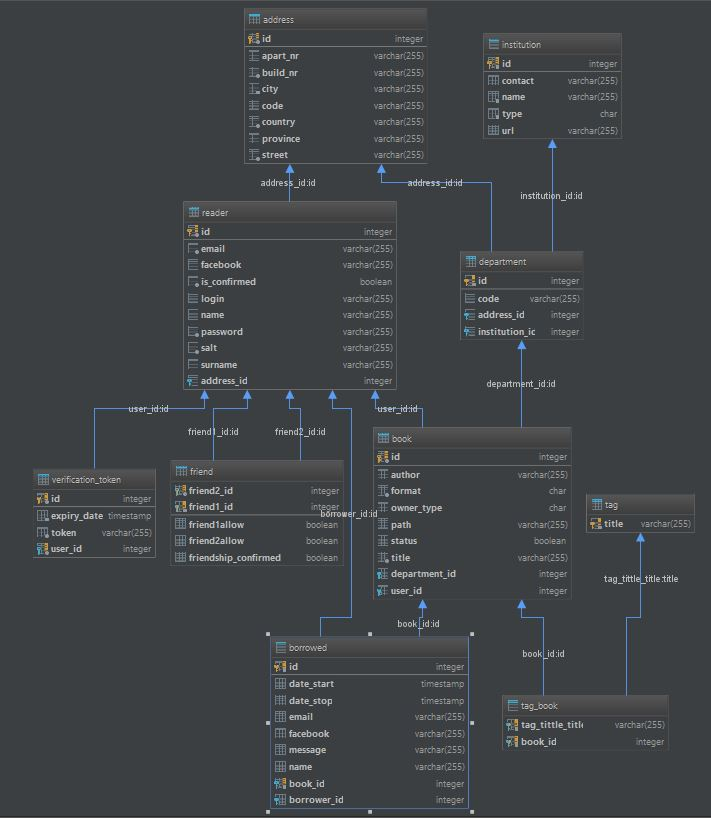
\includegraphics[width=1.\textwidth]{bookaDB.jpg}
			\end{figure}

\chapter{Opis techniczny}

	\section{Serwer aplikacji}
	
		\subsection{Podział aplikacji}
			
			\subsubsection{Kontroler}
			
			\subsubsection{Serwis}
			
			\subsubsection{Repozytorium}
			
		\subsection{System kont użytkowników}
		
			\subsubsection{Logowanie i sesja}
			
			\subsubsection{System pocztowy}
		
		\subsection{Przeszukiwanie zasobów bibliotecznych}
		
		
	\section{Aplikacja internetowa}
	
		%inne, jakiś tam podział na kontolery itp.
	
		\subsection{Kolejka komunikatów}
		
		\subsection{Google Drive}
	
	\section{Baza danych}
	
		%POJO



\chapter{Opis funkcjonalny}

	\section{Instalacja i konfiguracja systemu}
	
	\section{Opis funkcjonalności}


\chapter{Spis tabel i obrazów}


\begingroup
\let\clearpage\relax
\listoffigures
\listoftables
\endgroup



\end{document}